\subsubsection{\stid{4.10} DataLib} 

\paragraph{Overview} 

The Data Libraries and Services Enabling Exascale Science (DataLib)
project has been pushing on three distinct and critical
aspects of successful storage and I/O technologies for ECP applications:
enhancing and enabling traditional I/O libraries used by DOE/ECP
codes on leadership platforms, establishing a nascent paradigm of data
services specialized for ECP codes, and working closely with facilities
to ensure the successful deployment of our tools. In FY20-23 we plan to
continue to focus on these three complementary aspects of storage and
I/O technologies, adjusting in response to changing needs and bringing
these three aspects together to provide the most capable products for
end users. DataLib activities ensure that facilities have key production
tools, including tools to debug I/O problems in ECP codes; enable multiple
I/O middleware packages through Mochi and ROMIO; and will provide high
performance implementations of major I/O APIs in use by ECP codes.

We strongly support ECP management’s shift of focus towards
\textbf{Hierarchical Data Format (HDF)}. In response to ECP guidance
to prioritize the HDF5 API, we propose to emphasize enhanced HDF5
capabilities for ECP codes on current and future DOE leadership
platforms, strengthening HDF as a core technology for the future. We
propose to shift our focus away from ROMIO and PnetCDF development work
to enable rapid progress on this topic. We will continue to support the
use of Mochi tools for development of data services and I/O middleware,
including assisting other ECP AD, ECP ST, and vendor teams in providing
the best storage services possible for ECP applications. We will also
continue to work closely with the facilities to ensure the availability
and quality of our tools on critical platforms.

The \textbf{Darshan} I/O characterization toolset is an instrumentation tool
deployed at facilities to capture information on I/O behavior of
applications running at scale on production systems. It has become
popular at many DOE facilities and is usually “on by default”. Darshan
data dramatically accelerates root cause analysis of performance
problems for applications and can also (in some cases) assist in
correctness debugging. Our work in this project focuses on extending
Darshan to new interfaces and ensuring readiness on upcoming
platforms.

The \textbf{ROMIO} and \textbf{Parallel netCDF} (PnetCDF) activities
focus on existing standards-based interfaces in broad use, assisting
in performance debugging on new platforms and augmenting existing
implementations to support new storage models (e.g., “burst
buffers”). In addition to being used directly by applications, ROMIO
and PnetCDF are also indirectly used in HDF5 and netCDF-4. Our work is
ensuring that these libraries are ready for upcoming platforms and
effective for their users (and ready as alternatives if other
libraries fall short).

The \textbf{Mochi} and \textbf{Mercury} software tools are building blocks for
user-level distributed HPC services. They address issues of
performance, programmability, and portability in this key facet of
data service development. Mercury is being used by Intel in the
development of their DAOS storage service and in other data service
activities, while within ECP the HXHIM and UnifyCR projects also have
plans to leverage these tools. In addition to working with these
stakeholders and ensuring performance and correctness on upcoming
platforms, we are also working with ECP application teams to customize
data services for their needs (e.g., memoization, ML model management
during learning). These are supporting tools that are not represented as 
official products in the ECP ST portfolio.

\paragraph{Key Challenges}

Each of these subprojects has its own set of challenges. Libraries
such as HDF, ROMIO, and PnetCDF have numerous users from over a decade of
production use, yet significant changes are needed to address the
scale, heterogeneity, and latency requirements of upcoming
applications. New algorithms and methods of storing data are required.
%
For Darshan, the challenge is to operate in a transparent manner in
the face of continuing change in build environments, to grow in
functionality to cover new interfaces while remaining ``lean'' from a
resource utilization perspective, and to interoperate with other tools
that use similar methods to hook into applications.
%
Mochi and Mercury are new tools, so the challenge in the context of
these tools is to find users, adapt and improve to better support
those users, and gain a foothold in the science community.

\paragraph{Solution Strategy}

\emph{HDF enhancement.} HDF is the most popular high-level API for
interacting with storage in the DOE complex, but users express concerns
with the current The HDF Group (THG) implementation. We propose to perform
an independent assessment and systematic software development activity
targeting the highest possible performance for users of the HDF5 API on
ECP platforms of interest.

\emph{Directly supporting ECP applications and facilities.} We currently
have ongoing interactions with E3SM (PnetCDF), CANDLE (FlameStore/Mochi),
and ATDM/Ristra (Quantaii/Mochi), and we routinely work with the
facilities as relates to Darshan deployments. Our work with these
teams is targeted on specific use cases that are inhibiting their use
of current pre-exascale systems, such as E3SM output at scale using the
netCDF-4/PIO/PnetCDF preferred code path. We will continue to work with
these teams to address concerns, to maintain portability and performance,
and may develop new capabilities if needs arise. 

\emph{Supporting data services.} Mochi framework components are in use in
multiple ECP related activities, including in the UnifyCR and Proactive
Data Containers (PDC) in ExaHDF5 (WBS 2.4.x) and in the Distributed
Asynchronous Object Storage and other services in the Intel storage
software stack. The VeloC and DataSpaces teams (WBS 2.4.x and x.y.z as
part of CODAR, respectively) are also strongly considering adoption
of our tools. Mochi components enhance the performance, portability,
and robustness of these packages, and our common reliance on Mochi
components means that as Mochi improves, so do all these users.

\emph{Integration and Software QA.} DataLib has actively pursued
integration with the ECP ST software stack through the development
and upstreaming of Spack packages and the development and deployment
of automated testing for DataLib technologies, so we are already well
positioned in this aspect of our work. We anticipate this effort to
continue throughout the FY20-23 timeframe, with the addition of pull
requests submitted to THG to upstream HDF5 enhancements and effort applied
to address identified issues in our technologies as appropriate.

\paragraph{Recent Progress}

\emph{STDM12-11:}
This milestone presents the deliverables of three new software features
in PnetCDF library: 1) making use of burst buffers to improve the
I/O performance; 2) providing read capability to HDF5 files; and 3)
providing read capability to BP files. The first feature aggregates
I/O requests transparently to burst buffers which are later flushed
to the parallel file system. This effectively achieve a better I/O
bandwidth utilization. The latter two features alleviates application
users from developing a separate set of I/O functions in order to read
files in HDF5 and BP formats. HDF5 has been a popular file format in the
scientific communities, with many third-party software packages for data
analysis and visualization. In addition to improve the productivity for
application scientists, these new features also encourage the PnetCDF user
communities, mainly in climate research, to expand to other scientific
disciplines.

\emph{STDM12-12:}
This milestone presents a Mercury suite release including
platform-independent fault detection mechanisms for providing fault
tolerance to ECP applications and data services. Additionally, a
demonstration of this functionality on a production platform relevant
to ECP and integration of correctness testing for this functionality
into Mercury suite regression testing.

\emph{STDM12-13:}
This milestone presents a Darshan software release including fine-grained
I/O tracing capabilities, with a mechanism to automatically enable tracing
at runtime. Additionally, we demonstrate the utility of this new automatic
tracing mechanism for gaining insights into an ECP application. The new
trace triggering mechanism provides Darshan users more control over
what files Darshan traces at runtime. Specifically, Darshan now allows
users to expose a file describing a set of trace triggers that control
whether or not tracing should be enabled for a particular file. Currently
supported triggers include static triggers that use filename-based or
MPI rank-based regex matching (i.e., filenames with a specific extension
or directory prefix, or files opened by a particular range of ranks),
as well as dynamic triggers based on access characteristics to files at
runtime (i.e., trace all files that had at least 50 percent accesses that were
small or unaligned).  

\emph{STDM12-14:}
In this milestone we demonstrate new two-phase I/O strategies in ROMIO. 
We took a two-pronged approach to meeting this milestone. ROMIO has been a
fundamental component of the HPC I/O stack for two decades. The original
“two-phase collective buffering” optimization has served us well,
but is beginning to show some design challenges on newest architectures
and scales. We also developed a service-based I/O provider, through which
we can deliver and explore I/O strategies in MPI and other contexts. 
Some ROMIO changes could be incorporated directly into MPICH and will be
available in the upcoming MPICH-3.3 release. Other changes are awaiting
review before inclusion. Benvolio  our service-oriented I/O provider,
is running on Theta, Argonne’s pre-exascale machine. We have developed
a ROMIO  driver , allowing us to evaluate Benvolio with standard MPI-I/O
benchmarks such as IOR. 

\emph{STDM12-21:}
Delivery of composable data services for the ParSplice ECP EXALT
application including source code changes to ParSplice and demonstration
 of use including performance analysis on an HPC system.   The
Parallel Trajectory Splicing (ParSplice) application uses a novel
time-parallelization strategy for accelerated molecular dynamics. The
ParSplice technique (and associated application) enables long-time
scale molecular dynamics (MD) simulations of complex molecular systems
by employing a Markovian chaining approach allowing many independent MD
simulations to run concurrently to identify short trajectories called
“segments” that are then spliced together to create a trajectory
that spans long time scales. A master/worker approach is used to generate
segments starting from a set of initial coordinates stored in a key/value
database. From these initial coordinates the workers use traditional MD
simulation to generate a new segment and upon completion stores the final
coordinate of the segment in a distributed key/value database. Segments
are keyed by their atomic coordinates (corresponding to local energy
minima) while the value is simulation state information associated with
this atomic coordinate.  Our work included the integration of a number
of composable data services developed within the Mochi ASCR project .

\begin{figure}[htb]
        \centering
        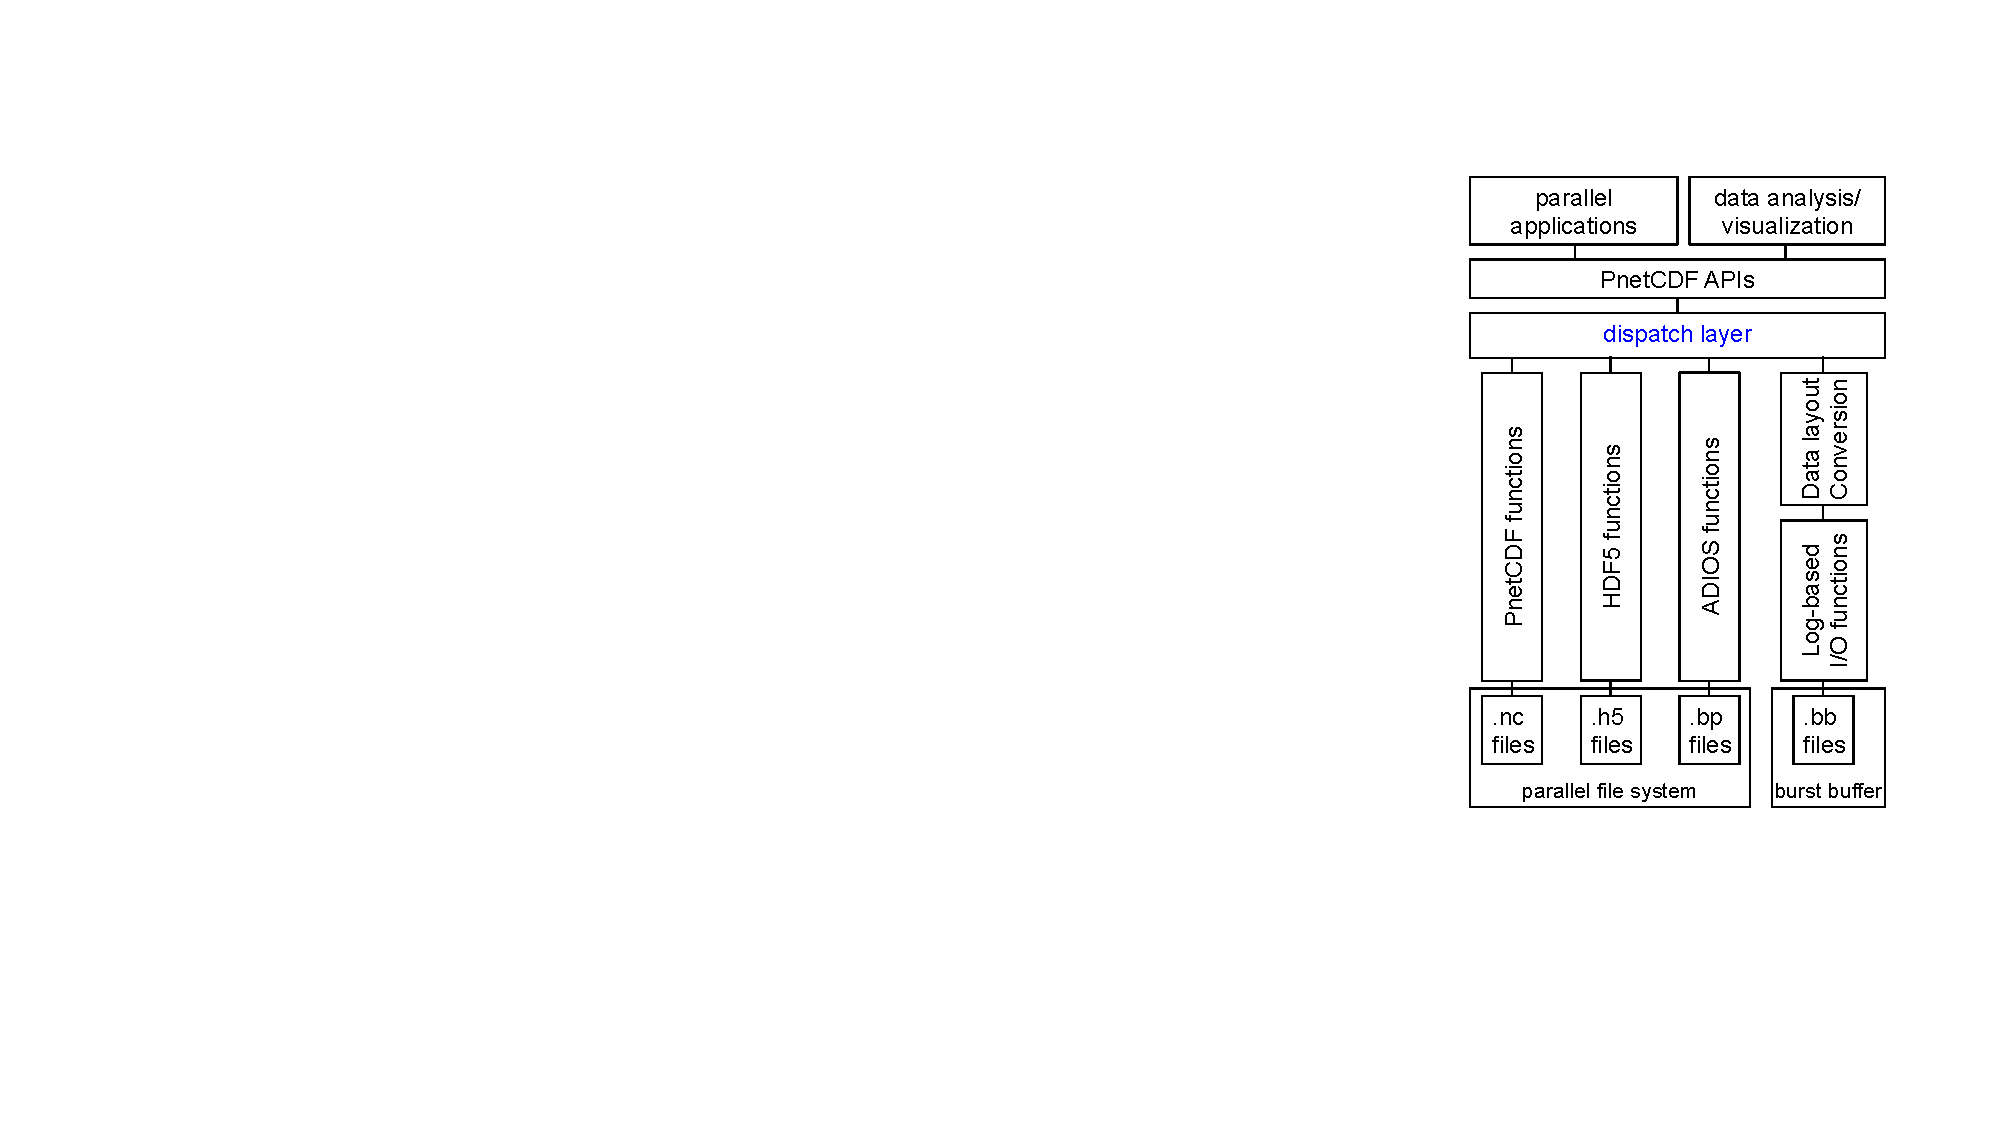
\includegraphics[height=2.5in]{projects/2.3.4-DataViz/2.3.4.10-DataLib/pnetcdf-figure.pdf}
        \caption{\label{fig:pnetcdf} The new PnetCDF dispatch layer provides flexibility to target different back-end formats and devices under the PnetCDF API used by many existing applications.
        }
\end{figure}

\paragraph{Next Steps}

Our plan for FY20 includes:
\begin{itemize}
\item Augmentation of our Darshan tool to capture API use at an
HDF5 dataset level of detail, building on existing (limited) HDF5
instrumentation. This enhancement will enable a better understanding of
codes using the HDF5 API across all domains, applications, and platforms,
facilitating more targeted and prioritized responses to performance
and/or reliability challenges.

\item Initial performance and overhead characterization using specific
ECP application workloads. Combined with detailed data from Darshan,
this activity will prepare us to best address ECP needs and also help
validate our initial approach. Users will be prioritized by potential
impact (e.g., supporting AMReX would impact multiple code teams),
prioritization by facilities (e.g., HACC is also an early science code
at ALCF), and ECP management input.

\item Design of an HDF5 VOL plug-in targeting ECP code requirements and a
specific platform and file system. The back-end file layout used in HDF5
is a known performance problem. We are confident that we can begin to
develop an alternative back end using modern parallel I/O concepts while
simultaneously performing the more comprehensive assessment described
above.

\item Further development and extension of FlameStore DNN model store
for CANDLE application.

\item	Development of Quantaii/Mochi to efficiently store, organize,
and index FleCSI data structures for ATDM/Ristra.

\item Exploration of E3SM HDF5 code paths and optimizations for key
checkpoint and analysis workloads.

\item Establishment of videoconferences with consumers of Mochi
technologies. This will enable us to more quickly respond to needs of
our stakeholders within ECP and vendors. 

\item Increasing stakeholder input on prioritization of Mochi technologies
and functionality. We will leverage the above mentioned videoconferences
as a tool for gathering stakeholder input on our Mochi development
activities, and we will adjust our plan going forward in response.

\item Integration of Darshan logging into HDF5 implementation as needed,
with any necessary modifications submitted to THG.

\item Extension of regular testing of Mochi tools to SummitDev test platform.
\end{itemize}
